\documentclass[12pt]{article}

\usepackage{graphics}
\usepackage{epsfig}
\usepackage{times}
\usepackage{amsmath}
\usepackage{wrapfig}

% <http://psl.cs.columbia.edu/phdczar/proposal.html>:
%
% The standard departmental thesis proposal format is the following:
%        30 pages
%        12 point type
%        1 inch margins all around = 6.5   inch column
%        (Total:  30 * 6.5   = 195 page-inches)
%
% For letter-size paper: 8.5 in x 11 in
% Latex Origin is 1''/1'', so measurements are relative to this.

\topmargin      0.0in
\headheight     0.0in
\headsep        0.0in
\oddsidemargin  0.0in
\evensidemargin 0.0in
\textheight     9.0in
\textwidth      6.5in

\title{{\bf Portable and Performant GPU/Heterogeneous Asynchronous Many-Task Runtime System} \\
\it Thesis proposal}
\author{ {\bf Brad Peterson}  \\
{\small bpeterson@sci.utah.edu}
}
\date{\today}

\begin{document}
\pagestyle{plain}
\pagenumbering{roman}
\maketitle

\pagebreak
\begin{abstract}

Asynchronous many-task (AMT) frameworks are maturing as a model for computing simulations on a diverse range of architectures at large-scale.  The Uintah AMT framework is driven by a philosophy of maintaining an application layer distinct from the underlying runtime while operating on an adaptive mesh grid.  This model has enabled task developers to focus on writing task code while minimizing their interaction with MPI transfers, halo processing, data stores, coherency of simulation variables, and proper ordering of task execution.   Uintah is also exploring portability using Kokkos for task code constructs along with a generalized Uintah API.  

Nvidia GPUs introduce numerous challenges in maintaining this clear separation between the application and runtime layer.  Specifically, Nvidia GPUs require code adhere to a proprietary programming model, use separate high capacity memory, utilize asynchrony of data movement and execution, and partition execution units among many streaming multiprocessors.  Abstracting these GPU features into an application layer requires numerous novel solutions to both Uintah and Kokkos.  

The focus of this research is largely split into two main parts, performance and portability.  Runtime performance comes from 1) minimizing runtime overhead when preparing simulation variables for tasks prior to execution, and 2) executing a heterogeneous mixture of tasks to keep compute node processing units busy.  Preparation of simulation variables, especially halo processing, receives significant emphasis as Uintah's target problems heavily rely on local and global halos.  In addition, this work covers automated data movement of simulation variables between host and GPU memory as well as distributing tasks throughout a GPU for execution.   This work does not describe strategies for optimizing task code, as that is an application developer responsibility.  Rather, this work enables application developers to achieve good wall time performance with low runtime overhead.   

Portability is becoming an productivity necessity for Uintah.  Application developers struggle to maintain three sets of code per task, namely code for single CPU core execution, CUDA code for GPU tasks, and a third set of code for Xeon Phi parallel execution.  Uintah seeks a portable solution through 1) unifying Uintah API for CPU and GPU tasks, and 2) adopting Kokkos as a portability layer enabling developers to write task code once while maintaining performance. Currently, Kokkos only supports synchronous GPU data copies and code execution.  Kokkos itself must be modified for asynchrony to performantly execute GPU tasks in Uintah's AMT runtime.  This research will cover both Uintah API and Kokkos changes and demonstrate results by applying these changes to production ready tasks.  
   
An overview of other runtimes and parallel tools is given in Chapter \ref{ch:related}.  Chapter \ref{ch:uintah_prior} describes the prior state of Uintah's GPU runtime.  Chapter \ref{ch:uintah_current} outlines work completed to date.  Chapter \ref{ch:workplan} provides remaining work required to meet the full goal of this thesis.  Chapter \ref{ch:thesis_format} outlines the proposed thesis format.  Chapter \ref{ch:thesis_plan} gives a thesis plan.  The remainder of this document contains the conclusion, references, and a list of my publications.   

\end{abstract}

\pagebreak
\tableofcontents
\pagebreak

\cleardoublepage
\pagenumbering{arabic}

%\section{Introduction}
%\label{ch:intro}


%This part provides an overall introduction of your work, including
%related work of your proposal.

\section{Existing Runtime Systems and Parallel Tools}
\label{ch:related}

AMT runtimes that have demonstrated scalability at large-scale or plan to reach that goal use varied approaches to aid application developers in their GPU implementations.   No clear dominant pattern has emerged.  Rather, these projects are motivated both by target problems and intended audiences which largely drive their priorities and accompanying abstractions.  Likewise, many parallel tools aiding developer productivity also take varied approaches to support targeted applications.  This chapter provides an overview of Uintah and its comparisons with other related AMT runtimes and tools.  

\subsection{Uintah and other AMT Runtimes}
\label{ch:amt_runtimes}

 
\begin{table}[]
	\centering
	\begin{tabular}{l|llllll}
		\cline{2-7}
        & \multicolumn{6}{c|}{Asynchronous Many-Task Runtimes}  \\ \cline{2-7}
		
		& \multicolumn{1}{c|}{Uintah}
		                                                       & \multicolumn{1}{c|}{Charm++}                               & \multicolumn{1}{c|}{Legion}                                & \multicolumn{1}{c|}{HPX}                                   & \multicolumn{1}{c|}{PaRSEC}                              & \multicolumn{1}{l|}{StarPU}                              \\ \hline
		\multicolumn{1}{|l|}{Common  usage}                                                                     & \begin{tabular}[c]{@{}l@{}}Multiphysics\\ on an adaptive\\ mesh grid\end{tabular} & \begin{tabular}[c]{@{}l@{}}Generalized\\ tool\end{tabular} & \begin{tabular}[c]{@{}l@{}}Generalized\\ tool\end{tabular} & \begin{tabular}[c]{@{}l@{}}Generalized\\ tool\end{tabular} & \begin{tabular}[c]{@{}l@{}}Linear\\ algebra\end{tabular} & \begin{tabular}[c]{@{}l@{}}Linear\\ algebra\end{tabular} \\ \cline{1-1}
		\multicolumn{1}{|l|}{\begin{tabular}[c]{@{}l@{}}Developer\\  involvement\\ with runtime\end{tabular}}   & Light                                                                             & Medium                                                     & Heavy                                                      & Medium                                                     & Medium                                                   & Medium                                                   \\ \cline{1-1}
		\multicolumn{1}{|l|}{\begin{tabular}[c]{@{}l@{}}Automatic\\  internodal\\  data movement\end{tabular}}  & Yes                                                                               & \begin{tabular}[c]{@{}l@{}}Invoked \\ by user\end{tabular} & Yes                                                        & Yes                                                        & Yes                                                      & No                                                       \\ \cline{1-1}
		\multicolumn{1}{|l|}{\begin{tabular}[c]{@{}l@{}}Automatic halo\\ gathering\end{tabular}}                & \begin{tabular}[c]{@{}l@{}}Host memory\\ (This work \\ for GPU)\end{tabular}      & No                                                         & Yes                                                        & No                                                         & Yes                                                      & No                                                       \\ \cline{1-1}
		\multicolumn{1}{|l|}{\begin{tabular}[c]{@{}l@{}}Data store \\ for application\\ developer\end{tabular}} & \begin{tabular}[c]{@{}l@{}}Host memory\\ (This work \\ for GPU)\end{tabular}      & No                                                         & No                                                         & No                                                         & No                                                       & No                                                       \\ \cline{1-1}
		\multicolumn{1}{|l|}{\begin{tabular}[c]{@{}l@{}}Automatic data\\ sharing among\\ tasks\end{tabular}}    & This work                                                                         & No                                                         & Yes                                                        & No                                                         & Yes                                                      & Yes                                                      \\ \cline{1-1}
		\multicolumn{1}{|l|}{GPU support}                                                                       & Yes                                                                               & \begin{tabular}[c]{@{}l@{}}With\\  add-ons\end{tabular}    & Yes                                                        & No                                                         & Yes                                                      & Yes                                                      \\ \cline{1-1}
		\multicolumn{1}{|l|}{\begin{tabular}[c]{@{}l@{}}Portable code \\ for CPU\\ and GPU tasks\end{tabular}}  & This work                                                                         & Weak                                                       & No                                                         & No                                                         & No                                                       & No                                                       \\ \cline{1-1}
	\end{tabular}
	\caption{A comparison of features of many current AMT runtimes }
	\label{table:runtimes}

\end{table}

A summary of several AMT runtimes is given in Table \ref{table:runtimes}.   Uintah ~\cite{MB-UUSCI-2012-001,wolfhpc12}  is unique among these runtimes in its combination of three high level goals 1) separating the application developer from the runtime through automated data stores and halo transfers, 2) support for a mixture of problems containing both local halo and global or nearly global halos and across multiple adaptive mesh refinement (AMR) levels, and (3) ability to reach full scale on current machines like Titan.  Further, Uintah's target problems operate on a 3D adaptive mesh grid, whereas the other runtimes seek for a more generalized solution not dependent on a mesh grid.  

Uintah supports problems where a compute node can have thousands of tasks, thousands of simulation variables, and millions of data dependencies both locally and globally across many levels of an AMR grid~\cite{espm2-brad}.  Uintah has been shown to scale to 16K nodes using GPUs on Titan~\cite{uintah-2016-titan-scaling} and 768K cores on Mira~\cite{uintah-2016-mira-scaling}.   In a search of literature, we found that Legion has been demonstrated to scale to 8K nodes on Titan~\cite{legion-2014-thesis-scaling}, Charm++ to 512K cores on Mira~\cite{charmpp-2017-scaling}, HPX to 1K nodes~\cite{HPX-scaling-global-address-space}, PaRSEC to 23,868 cores on Kraken~\cite{parsec-2014-scaling}, and StarPU to 256 nodes on the Occigen cluster located at CINES, France~\cite{starpu-2016-scaling}.  To the best of our knowledge, no other runtime can support such large, globally coupled problems with minimal application developer interaction.  

\begin{wrapfigure}{r}{8cm}
	\centering
	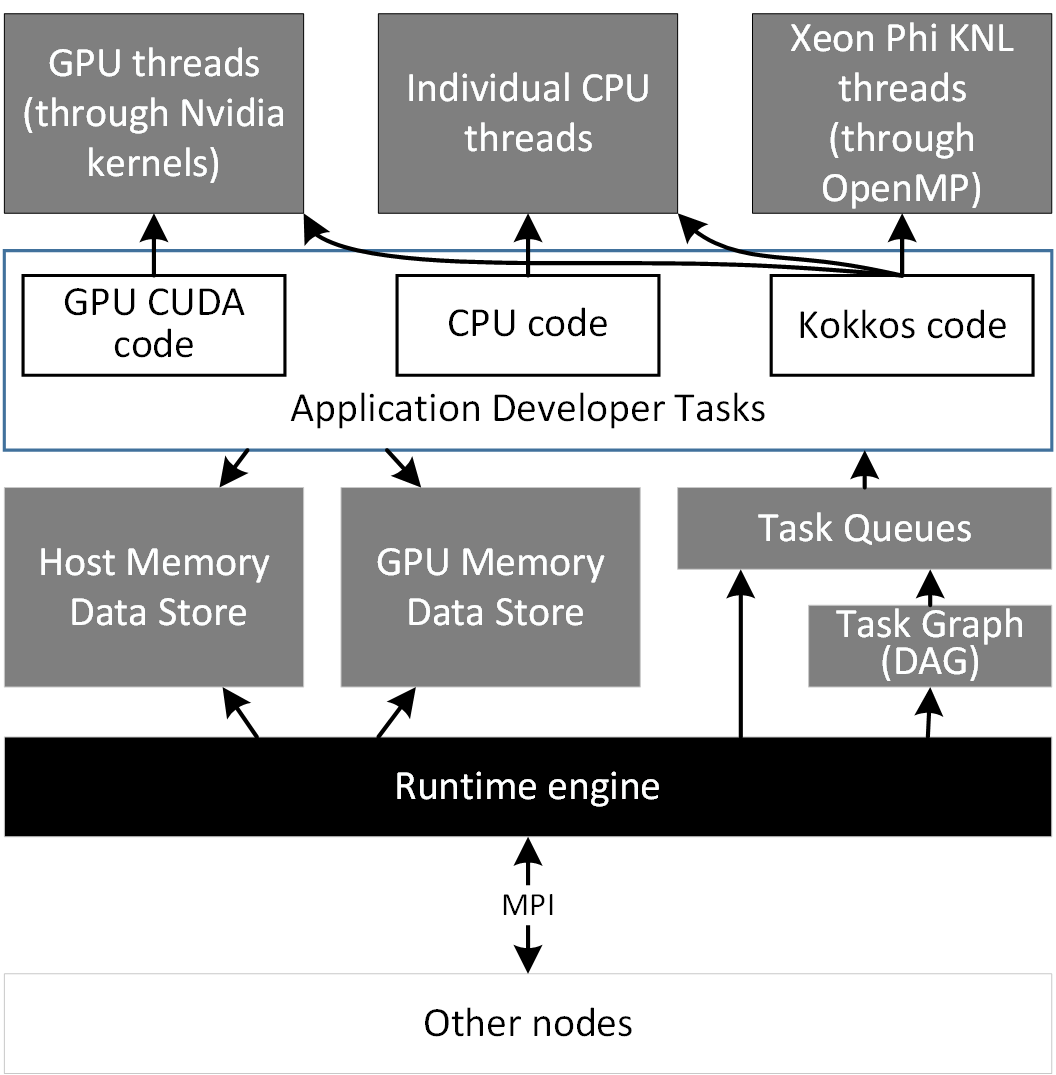
\includegraphics[width=8cm]{figures/Uintah_modules_simplified.png}
	\caption{Organization of major components and modules comprising Uintah}
	\label{fig:uintah-structure}
\end{wrapfigure}
 




Uintah is structured at a high level as shown in Figure \ref{fig:uintah-structure}. Uintah application developers supply task descriptions indicating all simulation variables required (including any needed halo cells) and the entry function necessary to execute the task.  An example task is shown in Figure \ref{fig:stencil27-task}.  That task's code will be found in the \emph{Stencil27::taskMethod()} function, and that task code may be CPU code, GPU CUDA code, or Kokkos parallel code.  In the task declaration, had the application developer not specified \emph{Ghost::AroundNodes, 1} for one cell layer of halo dependencies for that simulation variable, but rather \emph{Ghost::AroundNodes, 100} or \emph{Ghost::AroundNodes, 32767}, Uintah would automatically handle all halo management on a nearly global or global scale.  After all tasks are defined, the Uintah runtime processes these tasks into a distributed directed acyclic graph (DAG) of tasks.  Prior to task execution, the runtime prepares task simulation variables by issuing MPI sends and receives, and then gathers all halo data into simulation variables in host and GPU memory.  A task flows through various queues as its simulation variables are prepared and the task staged for execution.  The task itself can retrieve simulation variables from the data stores, further aiding application developer productivity.


\begin{wrapfigure}[12]{R}{8cm}
	\centering
	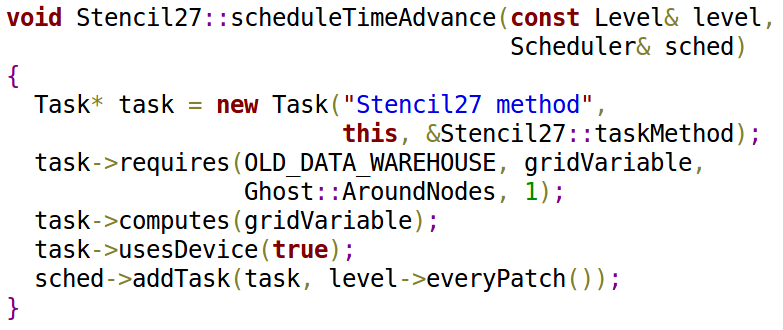
\includegraphics[width=8cm]{figures/stencil27-task.png}
	\caption{A Uintah task declaration which informs the runtime of a 27-point GPU stencil computation on a single Uintah grid variable.}
	\label{fig:stencil27-task}
\end{wrapfigure}



\subsubsection{Charm++}
\label{ch:charmpp}
Charm++~\cite{charmpp1993} is designed for a wide audience as a large, monolithic tool aiding developers requiring a prebuilt, mature, AMT runtime. Central to Charm++'s theme is their notion of message passing between tasks.  Charm++ does not explicitly define tasks and does not have a task graph, but rather relies on an event driven, message passing interface using callback functions.  When some code unit completes, the developer is responsible for invoking the message to the runtime providing the next function to invoke.  

Data movement to GPU memory and GPU code execution can be realized through their GPU Manager~\cite{charmpp-masters-gpumanager}.   While it is automatic in the sense that the GPU Manager will allocate GPU memory and perform host-to-GPU and GPU-to-host copies, the amount of development steps required to perform these steps are effectively equivalent to performing them through native CUDA code.  The GPU Manager requires the user provide their own CUDA kernels, amount of GPU memory buffers, and size of each buffer.  The user is also responsible for providing a callback functions when a GPU kernel completes.   Data copies and kernel execution can be realized asynchronously to support overlapping kernels.  The Accel framework~\cite{charmpp-thesis-accel} works on top of the GPU Manager and seeks to provide automatic CUDA kernel code generation, but its feature set is limited by effectively attempting to compile the same C++ code on a CPU compiler and then compiling it a second time on a CUDA compiler.

\subsubsection{Legion}
\label{ch:legion}
The Legion~\cite{legion2012} runtime system handles automatic dependency management and concurrency by first requiring the application developer supply many more characteristics of a data structure's data dependencies.  The application developer is expected to have a solid understanding of Legion's theoretical framework and extensive API to properly code application tasks that interact with the runtime.  Where Uintah seeks ease of development for application developers, Legion insists developers retain as much control over parallelism and data movement as possible.  

\subsubsection{HPX}
\label{ch:hpx}
The HPX runtime~\cite{HPX-scaling-global-address-space} recently reached version 1.0 but still awaits the introduction of many important features.  Its design strategy is both theoretical and bottom-up with the goal of providing a general asynchronous many-task runtime solution that is highly dependent on existing and forthcoming C++ standards.   HPX uses task scheduling and message passing to enable asynchrony and proper ordering of tasks.  At the moment, HPX has no built-in support for GPUs, data stores, automatic data dependency analysis, halo scattering and gathering, etc.   Internodal memory movement is achieved through a global address space.

\subsubsection{PaRSEC}
\label{ch:PaRSEC}
PaRSEC~\cite{parsec2012} contains many similarities with Uintah in that the runtime automates data transfer both through MPI for internode communication and between host and GPU memory for intranode communication.  In PaRSEC, data coherence utilizes a simplified version of the MOESI cache coherency protocol~\cite{parsec-coherency}.  Data dependencies are expressed by defining data flows among tasks using their customized JDF Format to help generate PaRSEC's DAG.  If MPI is used, the user provides nodal communication information through a process patterned after MPI\_Datatypes. 

\subsubsection{StarPU}
\label{ch:StarPU}
StarPU \cite{starpu} manages data copying and data coherency in different memory spaces using a process very similar to cache coherency protocols.  Halo transfers must be accomplished through user defined tasks.  For example, in a stencil-27 problem on a structured grid, transfering one cell layer of halo data would require 27 additional tasks.  Some application developer interaction is required to aid StarPU in MPI transfers among nodes.  

\subsection{Parallel Tools}
\label{ch:parallel_tools}

Many tools exist to aid application developer productivity in abstracting the complexities involved with parallel programming.  These tools may seek cleaner solutions for code portability, code simplification, or memory management in multiple memory hierarchies.  AMTs may choose to utilize these tools to fulfill a specific need not yet met by that runtime. 

When a Uintah task is executed, the runtime executes the user supplied task entry function.  Current application developers supply serial C++ code for CPU and Xeon Phi tasks and CUDA parallel code for GPU tasks.  That entry function could utilize other parallel tools such as OpenCL \cite{opencl-specification}, OpenACC \cite{openacc-25}, OpenMP \cite{openmp}, Raja \cite{raja}, or Kokkos \cite{kokkos2012}.  Uintah application developers have not used OpenCL as its performance often lags behind CUDA code \cite{Sorman2016}.  OpenACC has not been used as it offers no portability with the Xeon Phi KNL.  OpenMP 4.0 is performant on Xeon Phi KNLs, but it does not offer Uintah a fully portable solution as current GPU implementations are limited and lacking in GPU performance\cite{Martineau2016}.  Raja and Kokkos share high level similarities in utilizing lambda expressions for portability and performance with minimal disruptions to application developers.  Future Uintah work is focused on utilizing Kokkos as its current feature set is more extensive and mature.  

Regarding memory management, CUDA offers compelling features such as CUDA-aware MPI and Unified Memory to reduce the amount of temporary halo buffers and provides automatic memory movement between host and GPU memory.  Uintah does not restrict itself to only CUDA-aware MPI implementations, and Uintah provides automatic packed halo buffers which can then be made to work with GPUDirect if needed.  Uintah does not use Unified Memory as CUDA kernels operating in a Unified Memory environment demonstrate significantly slower execution times \cite{Landaverde2014AnIO}, and any GPU-to-host memory transfer requires a synchronization barrier prior to CUDA Compute Capability 6.x or expensive page faulting for Compute Capability 6.x \cite{nvidia-programming-guide-80}.  We desire performant kernels executing concurrently on numerous GPU streams without any synchronization and as a result we use the Uintah runtime to automate halo transfers and data movement between host and GPU memory without blocking operations.



\subsubsection{Kokkos}
\label{ch:Kokkos}
Kokkos~\cite{kokkos2012} describes itself as "a programming model in C++ for writing performance portable applications targeting all major HPC platforms. For that purpose, it provides abstractions for both parallel execution of code and data management. Kokkos is designed to target complex node architectures with N-level memory hierarchies and multiple types of execution resources. It currently can use OpenMP, Pthreads and CUDA as backend programming models."  The most fundamental component of Kokkos requires developers write functors or lambda expressions which are then placed inside a \texttt{parallel\_for}, \texttt{parallel\_reduce}, or \texttt{parallel\_scan} construct.  Alongside these parallel constructs are arguments specifying number of threads desired, execution patterns, and targeted execution space.  The architecture's compiler then compiles the functors and lambda expressions for the target architecture, and Kokkos will execute the functors or lambda expressions in the manner specified.  

The second major feature of Kokkos is aligning its parallel loops with the layout of data variables.  Kokkos maintains abstracted data objects supporting various layouts in up to 8 dimensions.   Kokkos Managed Views are data objects maintained by Kokkos itself, while Unmanaged Views are simply wrapped data pointers.  Managed Views have API to aid in copying data between memory spaces, such as host memory and GPU memory, but each host-to-GPU and GPU-to-host copy comes with the cost of a synchronization barrier.  Kokkos also maintains additional API to aid developers with portability libraries for atomic operations, locking mechanisms, basic task graph implementations, and random number generation.


  
Kokkos does not have any support for a concurrent data store interface, internode memory movement, automatic data gathering, asynchrony in data movement, heterogeneity in task scheduling, or overlapping of GPU execution.



\section{Uintah GPU Support Prior to This Research}
\label{ch:uintah_prior}

Prior Uintah work~\cite{wolfhpc12} provided a simplistic model for GPU task execution to target a reverse Monte Carlo Ray Tracing (RMCRT) component.  RMCRT tasks were long-lived (on the order or seconds to minutes) and required global or nearly global halos.  The prior work implemented rudimentary GPU data store (hereafter referred to as a Basic GPU Data Store) to enable \texttt{get()} API calls from within CUDA code.  Second, the task scheduler was modified by implementing four new steps.  1) Prepare the task by synchronously copying every task simulation variable from host memory to GPU memory. 2) Synchronously copy the entire Basic GPU Data Store managed in host memory into GPU memory.  3) Synchronously execute the GPU kernel found within the task.  4) Perform a cleanup phase where all computed simulation variables are synchronously copied back to host.  
	
This prior GPU execution model had numerous deficiencies for both portability and performance, and was only suitable for large monolithic problems executing properly blocked GPU kernels which computed in the order of seconds.  For all other simulations using Uintah, the combination of synchronization barriers, PCIe bus contention, and duplicated simulation variables meant that simulations utilizing GPU tasks either ran slower than their CPU counterparts, or they could not fit within GPU memory.  

\section{Current Work and Preliminary Results}
\label{ch:uintah_current}

Most of this chapter is summarized from work in my prior publications~\cite{saahpc-2010-brad, wolfhpc15,ijpp16, espm2-brad}.  The first publication describes experiences learned from storing particles on a mesh in GPU memory to achieve better performance.  The latter three publications describe work directly with Uintah itself enabling Uintah to open itself up to more classes of problems.  My work with Kokkos has not yet been submitted for publication.  

\subsection{GPU/Heterogenous Data Warehouses and Task Scheduler}
\label{ch:data warehouses}

The Wasatch project~\cite{wasatch-2015} and its accompanying Embedded Domain Specific Language (EDSL) called Nebo \cite{nebo_2015, sutherland_discrete_2011}, led by James Sutherland and Tony Saad, utilized Uintah with numerous short-lived GPU tasks which exposed performance flaws in the runtime.  The movement of many simulation variables into GPU memory and back to host memory took longer than the task execution.  However, most of this data movement was unnecessary as the only time simulation variables were required in host memory was to perform MPI sends and receives.  Uintah needed a solution that efficiently supported short-lived tasks with local halo transfers while also supporting the RMCRT component's long-lived tasks with global halo transfers.




\subsubsection{Processing Halo Data in GPU Memory}
\label{ch:processing_halo_data_gpu_memory}



A new GPU data store (GPU Data Warehouse) was implemented to give the Uintah runtime an expanded API to manage simulation variables in GPU memory~\cite{wolfhpc15}.  Simulation variables were also still tracked in the Basic GPU Data Store in host memory which would then be copied into GPU memory.  Several additional halo transferring scenarios were implemented (GPU-to-GPU, host-to-GPU, GPU-to-host, GPU-to-another MPI rank, another MPI rank-to-GPU). The Uintah runtime automatically performed all halo transfers for all scenarios.   Uintah launched CUDA kernels necessary to write data in or out of contiguous packed halo buffers.  For a sample Poisson problem, this new runtime engine improved simulation wall times with 2.82x to 5.39x speedups.   The cumulative effects of these changes for Wasatch tasks is seen in Figure~\ref{fig:wasatch-speedups}.  

\begin{figure}
	\centering
	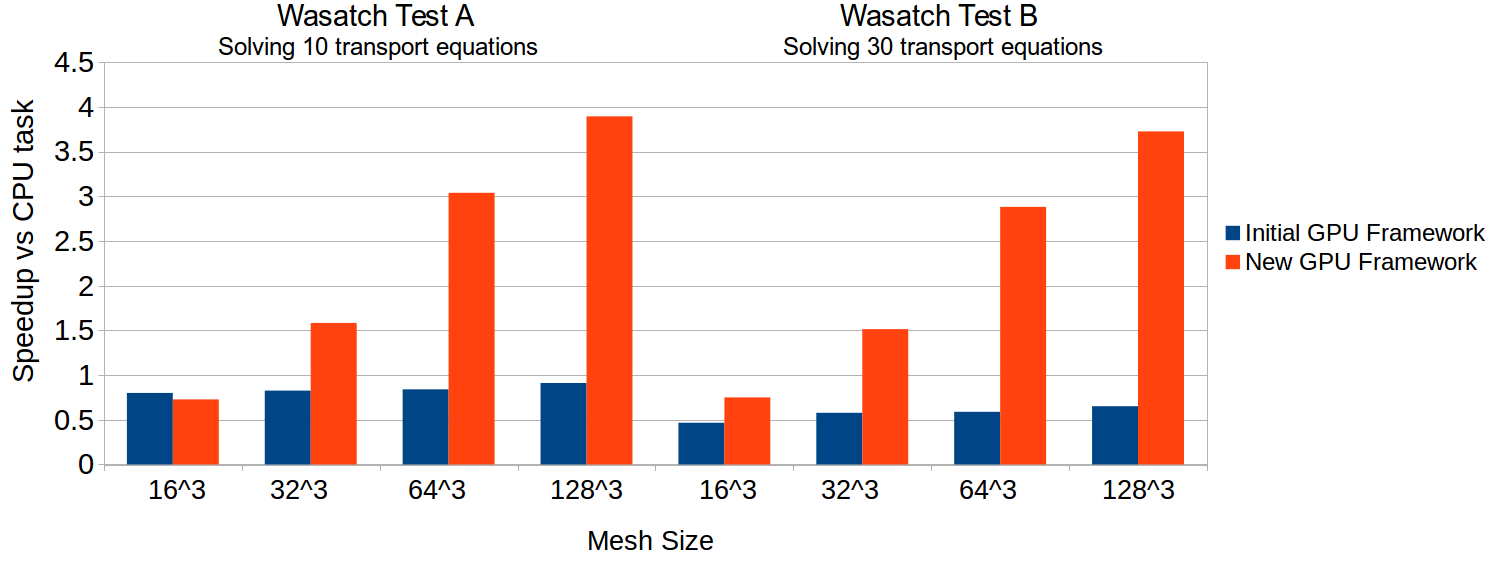
\includegraphics[width=0.70\textwidth]{figures/wasatch_test_bar_chart-highquality.png}
	\caption{Short-lived GPU tasks were most susceptible to runtime overhead.  Performing halo gathers entirely in GPU memory helped make total GPU simulation wall times tasks faster than CPU simulations.  Computations performed on an Nvidia GTX 680 GPU with CUDA 6.5 and an Intel Xeon E5-2620.}
	\label{fig:wasatch-speedups}
\end{figure}

\subsubsection{Simulation Variable Coherency}
\label{ch:simulation_variable_coherency}

An expanded task scheduler was paired with the GPU Data Warehouse to verify the status of any simulation variable in GPU memory.  The task scheduler prepared simulation variables prior to GPU task execution through allocation, host-to-GPU copies, and halo copies.  An atomic bitset was added to each simulation variable's entry in the GPU Data Warehouse to track a simulation variable's lifetime~\cite{ijpp16}.  Task scheduler threads coordinated with one another by atomically querying these bitsets to ensure no two threads prepared the same data action.  This change allowed the runtime to 1) simultaneously prepare two or more tasks sharing the same simulation variable, and 2) reduced memory usage in GPU memory.


\subsubsection{Task Data Stores}
\label{ch:task_data_warehouse}


Another GPU runtime enhancement reduced the size and enabled heterogeneous concurrency of the Basic GPU Data Store~\cite{wolfhpc15}.  The GPU Data Warehouse generated a Basic GPU Data Store giving each task its own version of the data store containing only the simulation variables it requires.  These data stores are termed Task Data Warehouses.   As shown in Figure~\ref{fig:task-data-warehouse}, the time spent copying data into GPU memory has been drastically reduced.  Task scheduler threads could copy Task Data Warehouses into GPU memory without interfering with each other, enabling full concurrency of GPU tasks by allowing kernel overlapping~\cite{ijpp16}.  Figure~\ref{fig:rmcrt-overlap} demonstrates this overlapping while running long-lived RMCRT tasks.  

\begin{figure}
	\centering
	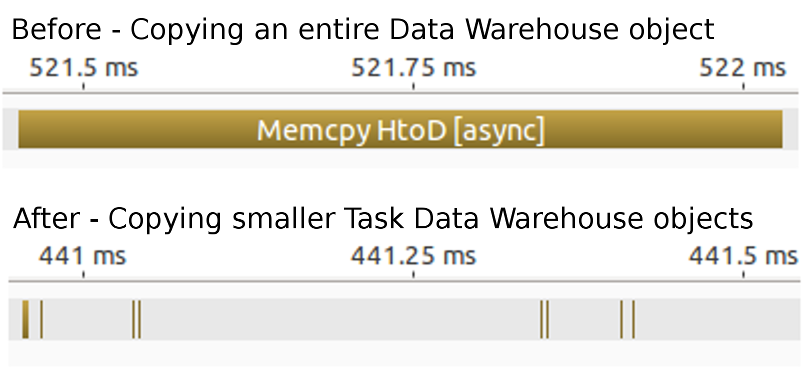
\includegraphics[width=0.80\textwidth]{figures/task_datawarehouse.png}
	\caption{Significant size reduction of Basic GPU Data Store objects better supports GPU tasks which execute on the order of milliseconds.  The Task Data Stores are not shared between tasks, enabling GPU task asynchrony and overlapping. }
	\label{fig:task-data-warehouse}
\end{figure}

\begin{figure}
	\centering
	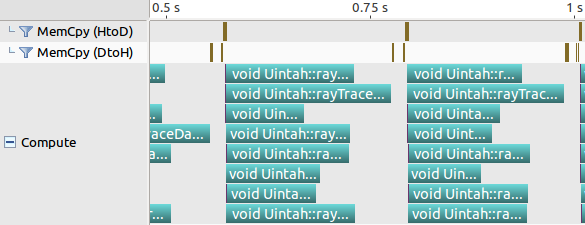
\includegraphics[width=0.80\textwidth]{figures/rmcrt_after_zoomed_sidebar.png}
	\caption{Data sharing and among tasks and GPU Task Data Stores allows the Uintah runtime to asynchronously invokes 16 sets of host-to-GPU copies followed by GPU task kernel executions.  Computations performed on 16 RMCRT tasks per time step on an Nvidia K20c GPU.}
	\label{fig:rmcrt-overlap}
\end{figure}

\subsubsection{Global Halos in the GPU Data Warehouse}
\label{ch:global_halos_gpu_data_warehouse}
The GPU Data Warehouse was further modified to avoid data duplication in the presence of global data dependencies.  This change was motivated by a recent production run on the DOE Titan supercomputer for a proposed high efficiency coal boiler.  The GPU Data Warehouse and accompanying task scheduler only supported tasks sharing simulation variables, but not sharing of halo data.  The GPU Data Warehouse was modified to allow multiple data warehouse entries to create and use a shared data object~\cite{espm2-brad}.  Likewise, task scheduler threads coordinated to ensure no two threads created duplicates of the shared data object.  The result of these changes reduced memory usage allowing the problem to fit into GPU memory as shown in Table~\ref{table:phase_times}.  The cumulative work described so far can be seen in Figure~\ref{fig:rmcrt-cumulative} as combined data warehouse and task scheduler has enabled substantial speedups.

	
\begin{table}[]
	\centering
	\begin{tabular}{|l|c|c|}
	\hline
	\multicolumn{3}{|c|}{Memory Overhead Improvements}                                                                                                                                                                                                                   \\ \hline
	Simulation patch layout                                                                                          & \begin{tabular}[c]{@{}c@{}}Host memory usage\\  before (MB)\end{tabular} & \begin{tabular}[c]{@{}c@{}}Host memory usage\\ after (MB)\end{tabular} \\ \hline
	\begin{tabular}[c]{@{}l@{}}Coarse: $32^3$ cells, $4^3$ patches\\ Fine: $64^3$ cells, $4^3$ patches\end{tabular}  & 3073                                                                     & 65                                                                     \\ \hline
	\begin{tabular}[c]{@{}l@{}}Coarse: $32^3$ cells, $4^3$ patches\\ Fine: $128^3$ cells, $4^3$ patches\end{tabular} & 23229                                                                    & 279                                                                    \\ \hline
	\begin{tabular}[c]{@{}l@{}}Coarse: $64^3$ cells, $4^3$ patches\\ Fine: $128^3$ cells, $4^3$patches\end{tabular}  & Exceeded memory                                                          & 311                                                                    \\ \hline
	\end{tabular}
	\caption{Memory reductions from sharing halo data among simulation variables.  Global data dependencies previously required each simulation variable to have its own copy of the entire domain.}
	\label{table:phase_times}
\end{table}



\begin{figure}
	\centering
	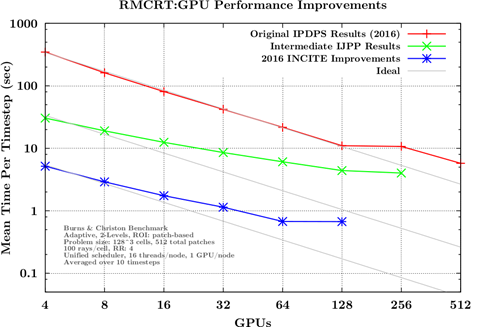
\includegraphics[width=0.70\textwidth]{figures/rmcrt-cumulative.png}
	\caption{Speedups of one to two orders of magnitude of the Uintah GPU runtime from before this work until December 2016.   }
	\label{fig:rmcrt-cumulative}
\end{figure}

\subsubsection{Distributing Tasks Among a GPU}
\label{ch:generalizing_task_execution}
Obtaining performance on GPUs is frequently achieved through many small blocks of kernel execution rather than large monolithic kernels.  The GPU can distribute many small kernels among all of its streaming multiprocessors (SMs).  Using Uintah to over-decompose a problem into finer execution units is difficult due to finding a suitable decomposition geometry and increased dependency analysis among many more tasks.  A solution was found~\cite{espm2-brad} where a task could split itself into many kernels, with each kernel executing on a different stream.  This modification enables Uintah to saturate a GPU no matter how many SMs it has.   Figure~\ref{fig:rmcrt-distributing-tasks} demonstrates that more kernels for a task do a better job of keeping a GPU occupied during a time step.    

\begin{figure}
	\centering
	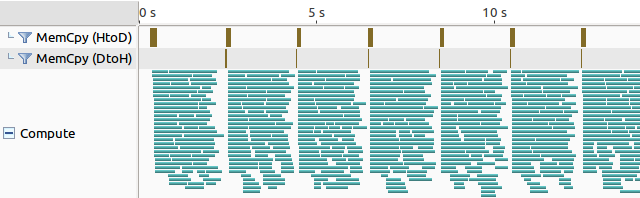
\includegraphics[width=0.60\textwidth]{figures/phaseiii-multistream-300rays-28x28x56_8threads_6streams_crop.png}
	\caption{Profile of a simulation which splits GPU tasks into many smaller kernels each with its own stream.  Computations performed on 16 RMCRT tasks per time step on a Nvidia K20c GPU.   }
	\label{fig:rmcrt-distributing-tasks}
\end{figure}




%\subsection{Reduction of Dependency Analysis}
%In preparation for the recent production coal boiler run, the Uintah runtime had major performance deficiencies analyzing all dependencies among nodes in the presence of global data dependencies.  Each task was responsible for determining what messages it must send out and what messages it must receive.  The first trial run of the production problem performed this analysis phase in 4.5 hours.  A dependency search algorithm was implemented to restrict dependency searches among tasks by finding maximum extents each task has within the simulation.  For example, a task that simply computes simulation variables does not specify any halo extents.  However, by analyzing how that simulation variable is used throughout other tasks, a vast swath of potential dependencies can be ruled out.  In the production problem, dependency analysis was reduced 93% to 20 minutes, with most of the remaining time due to an unrelated problem finding cell extents among multiple adaptive mesh refinement layers.    



\subsection{Modifying Kokkos for Asynchrony}
\label{ch:kokkos_modifications}
Kokkos's memory movement and kernel execution for Nvidia GPUs is similar to Uintah's GPU runtime two years ago.  CUDA barriers are used extensively to avoid concurrency issues.  Users using Kokkos must work with large, monolithic GPU kernels, which requires subdiving a functor into enough threads to properly fit within all GPU SMs.  This approach puts a difficult burden on application developers trying to properly size and partition problems.  Further, with Uintah usually running each task on a $16^3$ region of cells, it is difficult to subdivide such small regions to distribute throughout the GPU.  

\begin{figure}
	\centering
	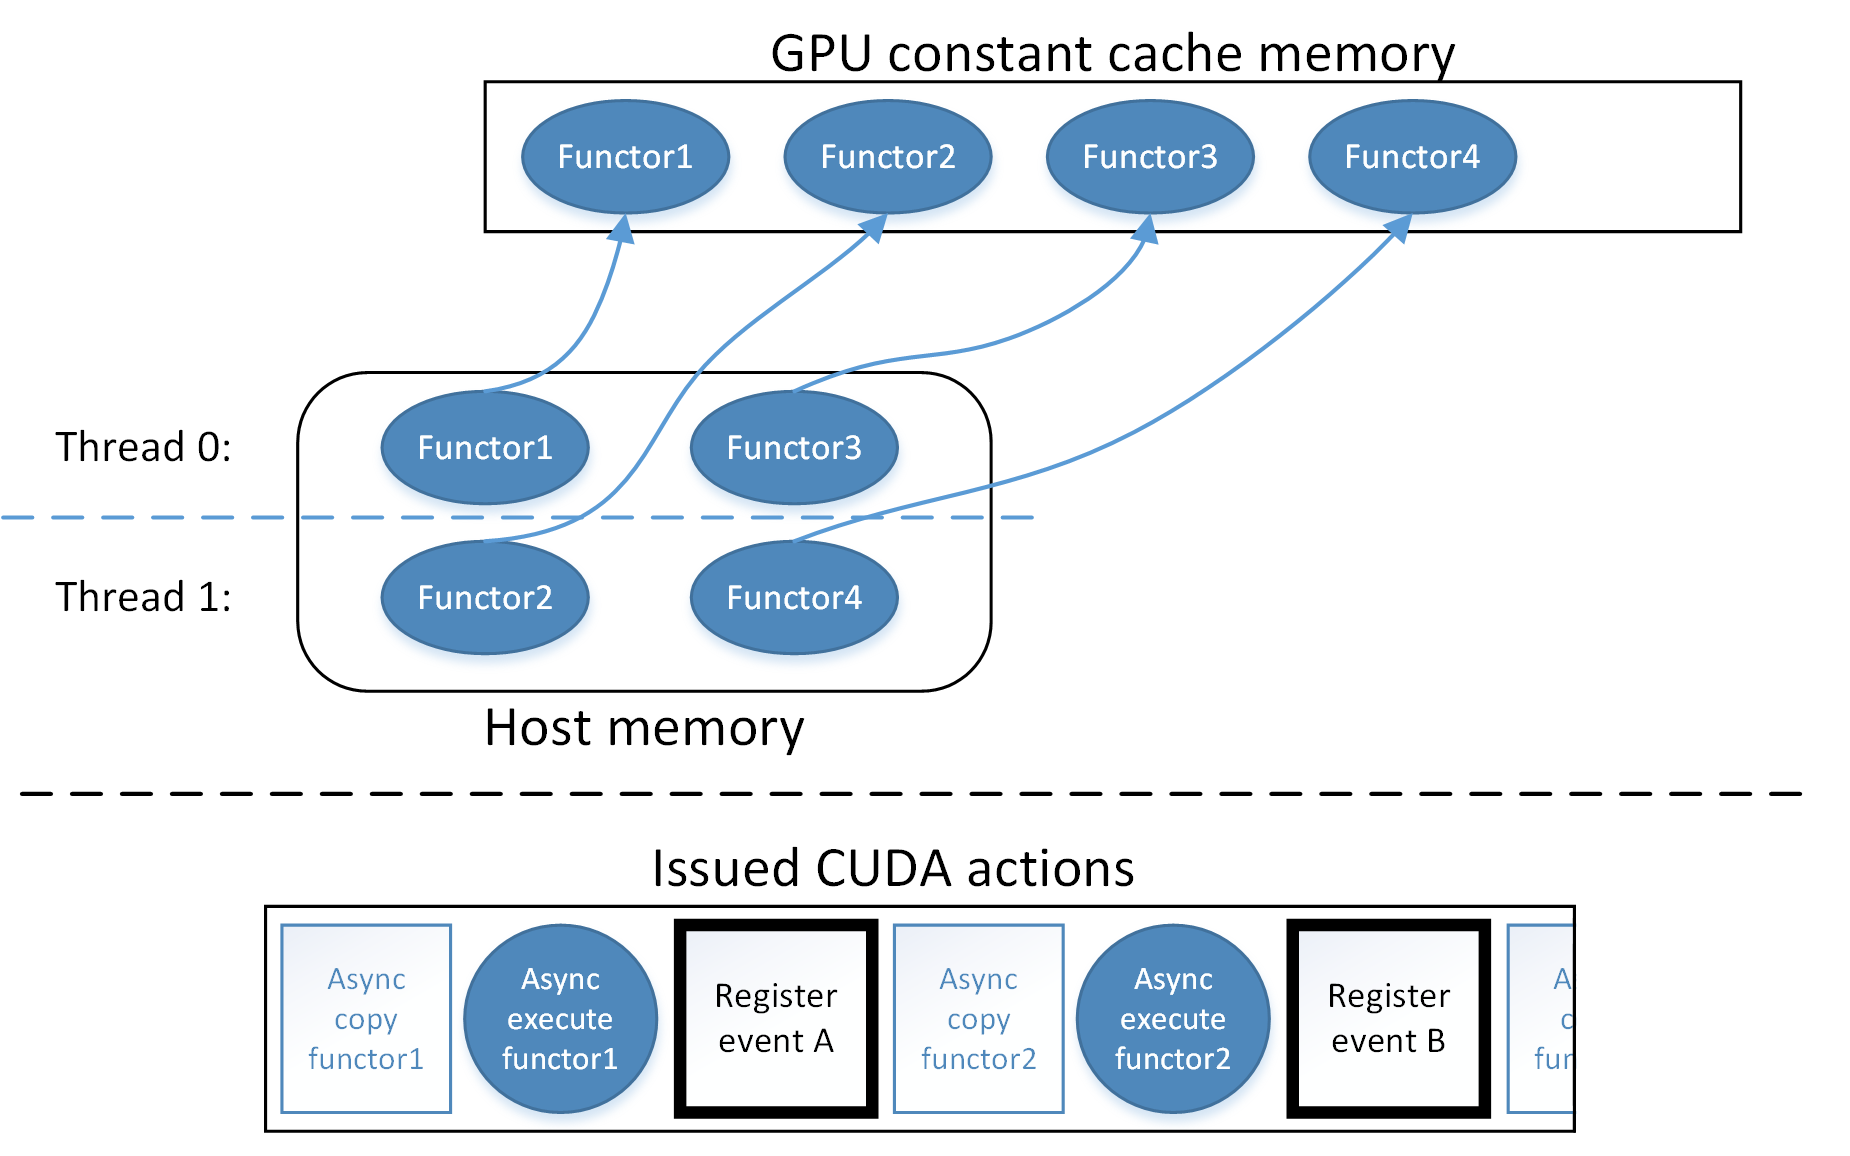
\includegraphics[width=0.60\textwidth]{figures/Kokkos_constant_cache_new.png}
	\caption{Data for multiple functors can be staged into GPU Constant memory, executed, and tracked with CUDA Events.   }
	\label{fig:kokkos-constant-cache-new}
\end{figure}

Recent work modified Kokkos to support asynchrony of Kokkos \texttt{parallel\_for} code.  Under-the-hood the Kokkos engine now allows multiple threads to claim a region of GPU constant cache memory, asynchronously copy the functor's information into that space, then launch the kernel to execute that functor.  A visual representation of this is given in Figure~\ref{fig:kokkos-constant-cache-new}.  CUDA streams themselves are encapsulated into Kokkos::Cuda objects, and reference counting ensures that when all instances of the object are destructed the stream itself is reclaimed.  This allows any application developer using Kokkos \texttt{parallel\_for} constructs to overlap kernels with only one minor modification to their existing code. 




\section{Future Work Plan and Implications}
\label{ch:workplan}

\subsection{Performance}
\label{ch:workplan-performance}
\subsubsection{Task Scheduler Modifications}
\label{ch:task-scheduler-modification}
Currently the Host Memory Data Warehouse allocates space on-the-fly during task execution for host memory simulation variables.  To support sharing data objects and a unified code base, this model must change so that simulation variables are allocated prior to task execution.   Any task simulation variables identified as computing a new value should be pre-sized for upcoming halo cells based on the what can be inferred.  Determining a proper size is a challenge as the initialization time step has no information as to what halo cells will soon be found in a normal time step.  Resizing variables in GPU memory may also be a messy process.  

\subsubsection{Halo Gathering}
\label{ch:workplan-halo-gathering}
Using packed contiguous buffers to transfer halo data is the correct approach~\cite{ijpp16} for Uintah's target problems operating on a 3D grid, however, Uintah's current implementation requires more fine tuning to reach this potential. Currently both James Sutherland and I have recognized unwanted performance deficiencies in the current approach of utilizing a GPU kernel to gather in halo cells.   The CUDA kernel is not operating at high efficiency, and some investigation is needed to reduce overhead of utilizing these packed halo buffers. 

\subsection{Portability}
\label{ch:workplan-portability}
\subsubsection{Unifying the Data Warehouses into One Codebase}
\label{ch:workplan-unified-data-warehouse}
The Host Memory Data Warehouse and the GPU Data Warehouse have very different philosophies which need to be merged into one codebase.  The Host Memory Data Warehouse largely avoids concurrency issues by duplicating simulation variables any time halo copying occurs or when two or more tasks share a simulation variable.  

As Uintah is heavily implemented with Host Memory Data Warehouse code throughout, future work will preserve this class and merge GPU Data Warehouse concurrency and data sharing functionality into it.  This may require making the underlying map data structure lock free.  This work may be troublesome as the Uintah codebase is large and complex, with numerous code hacks for various edge cases.  My initial assumption is that it's likely some developers will insist on backwards compatibility for their edge cases with their legacy code.

\subsubsection{Kokkos Modfications}
\label{ch:workplan-kokkos-modifications}
Uintah utilizes the Kokkos \texttt{parallel\_for} and \texttt{parallel\_reduce} constructs.  The work achieved for the \texttt{parallel\_for} and for CUDA GPU tasks needs further investigation and implementation into Kokkos.  The overall goal here is to deliver updates useful to the Kokkos project, and not just Uintah. 
\subsubsection{Uintah Integration with Kokkos}
\label{ch:workplan-kokkos-integration}
Results will be limited to existing tasks already written using CUDA code or Kokkos constructs.  This work plan will not attempt to rewrite any existing task into GPU or Kokkos code.   RMCRT is an excellent target problem for this research as we already have RMCRT code written for single threaded CPU, GPU, and Kokkos.  The Arches team has tasks written with CPU code and Kokkos code.  

\subsection{Limitations of Work Plan}
\label{ch:workplan-limitations}
Some limitations in upcoming work will likely occur as occasionally developers write tasks that conflict with Uintah philosophy.  Five examples are 1) developers writing CPU tasks occasionally allocate their own simulation variables and perform their own halo cell gathers using a \texttt{getRegion()} call. 2) Application developers sometimes perform a Data Warehouse \texttt{get()} API call despite the task not previously listing that simulation variable. 3) A task may attempt to obtain both a CPU and GPU data pointer.  4) Developers utilize Uintah templated simulation variables with non-standard types (e.g. a \texttt{CCVariable} with a custom container object).  5) CPU and Xeon Phi tasks make OS API calls which are unavailable to GPUs.  For these reasons, it is very unlikely this work can achieve a full production run of the recent coal boiler multiphysics simulation on GPUs.  This work instead will provide the mechanism so Kokkos enabled tasks can run on GPUs if properly designed.  


\section{Thesis Format}
\label{ch:thesis_format}

My proposed thesis structure is as follows:\\
\\
\textbf{ABSTRACT}\\
\textbf{CHAPTER 1 – Introduction}\\
A description for the motivation of this project, past contributions, and the prior state of Uintah's GPU functionality. This chapter will refer to past work done by others Uintah~\cite{wolfhpc12, meng-dissertation}.\\  
\textbf{CHAPTER 2 – Related Frameworks and Tools}\\
This chapter will be an expanded form of this document's overview of related tools and demonstrate the novelty of this research.\\  
\textbf{CHAPTER 3 – Uintah Overview and Application Developer API}\\
Chapter 3 will contain an overview of the many moving parts that enable Uintah to function.  A description will be given of all steps required for an application developer to create and execute CPU and GPU tasks.  \\  
\textbf{CHAPTER 4 -- A Host and GPU Data Store Enabling Concurrency, Asynchrony, and Data Sharing}\\ 
This chapter will use work from my prior publications~\cite{wolfhpc15,ijpp16,espm2-brad} and future work.  This chapter will contain an overview of the existing Host Memory Data Warehouse, including its strengths and limitations.  One section will cover the GPU Data Warehouse including its iterations, with a demonstration at each iteration what new characteristics it achieved.  This chapter should conclude with a data warehouse design using a unified codebase managing data in both host memory and GPU memory.\\  
\textbf{CHAPTER 5 – Uintah Heterogenous/GPU Task Scheduling and Execution}\\
This chapter will use work from my prior publications~\cite{wolfhpc15,ijpp16,espm2-brad} and future work.  
Task schedulers are the glue enabling the Uintah data store to achieve concurrency, asynchrony, and sharing of data.  This chapter will analyze and report the many steps of a task lifetime: simulation variable preparation, halo cell gathering, task execution, and task cleanup.\\ 
\textbf{CHAPTER 6 – Kokkos Code Modifications for Asynchrony of Data Movement and Execution}\\
This chapter will utilize current and future work~\cite{espm2-16,jocs18}.  Kokkos has strong potential as a portable code solution for Uintah, but its GPU performance is currently basic and limited.  In particular, Kokkos frequently utilizes synchronization barriers and has no mechanisms to support computation. This chapter will describe how Kokkos itself was modified to achieve full asynchrony.\\
\textbf{CHAPTER 7 – Kokkos and GPU Integration Into Uintah}\\
This chapter will utilize current and future work~\cite{espm2-16,jocs18}.  I desire this chapter to be the capstone of the dissertation, demonstrating both performance and portability using production scale multiphysics tasks, while simultaneously minimizing application developer interaction with specific architectures.  This chapter will highlight the ease which an application developer can create a task and performantly execute it on a GPU, CPU, or Xeon Phi KNL.  Some specific integration details are needed, such as transposing simulation variables and utilizing Kokkos Unmanaged Views.\\  
\textbf{CHAPTER 8 – Conclusions and Future work}\\
\textbf{APPENDIX}\\
\textbf{REFERENCES}\\

\section{Thesis Plan}
\label{ch:thesis_plan}

\textbf{November-December 2017}: Finish Kokkos work on \texttt{parallel\_for}, \texttt{parallel\_reduce}, and supporting tools.  Demonstrate Kokkos with RMCRT in Uintah with various code bases.  Write Abstract and Chapters 6 and 7 of the dissertation.\\
\\
\textbf{January 2018}: Begin transitioning to a unified data warehouse model.  This involves modifying the Host Memory Data Warehouse to use similar logic as the GPU model where allocations are done prior by the scheduler, and not during task execution by the application developer.  Finish Abstract, Chapter 1, 2, and 3.\\
\\
\textbf{February 2018}: Continue implementing changes for a unified Data Warehouse model.  Gather data necessary to fully write Chapter 4.\\
\\
\textbf{March 2018}: Continue implementing changes for a unified Data Warehouse model.  Gather data necessary to fully write Chapter 5.  \\
\\
\textbf{April 2018}: Finish all leftover work.  Print and bind into dissertation.  Defend. \\
\\
\textbf{May-June 2018}: Work with Thesis Office to complete and publish the dissertation. \\


\section{Conclusions}
\label{ch:conclusions}

The high-level goal of past and ongoing research is demonstrating both portability and performance of GPU enabled tasks for a production problem in the Uintah AMT runtime system.  The portability goal should preserve Uintah's philosophy of requiring minimal runtime API interaction with the application developer while allowing tasks written with Kokkos to run on multiple architectures.  The performance goal minimizes runtime wall time overhead and simulation variable duplication in memory.   When completed, this will make Uintah the first mature AMT runtime that has a combination of simulation variable management, GPU portability, performance, and ease of application task development. 

\section{Publications}

\cite{espm2-brad}  --- \textbf{B. Peterson}, A. Humphrey, J. Schmidt, M. Berzins.  "Addressing Global Data Dependencies in Heterogenous Asynchronous Runtime Systems on GPUs", In {Proceedings of the Third International Workshop on Extreme Scale Programming Models and Middleware (ESPM2'17)}, 2017. \\
\\
\cite{espm2-16}  --- D. Sunderland, \textbf{B. Peterson}, J. Schmidt, A. Humphrey, J. Thornock, and M. Berzins. "An Overview of Performance Portability in the Uintah Runtime System Through the Use of Kokkos."  In \textit{Proceedings of the Second International Workshop on Extreme Scale Programming Models and Middleware (ESPM2)}. IEEE Press, Piscataway, NJ, USA, 44-47. 2016.\\
\\
\cite{respa-techreport-15} --- \textbf{B. Peterson}, N. Xiao, J. Holmen, S. Chaganti, A. Pakki, J. Schmidt, D. Sunderland, A. Humphrey, M. Berzins. "Developing Uintah's Runtime System For Forthcoming Architectures," Subtitled "Refereed paper presented at the RESPA 15 Workshop at SuperComputing 2015 Austin Texas," \textit{SCI Institute}, 2015.\\
\\
\cite{wolfhpc15} --- \textbf{B. Peterson}, A. Humphrey, H. K. Dasari, J.C. Sutherland, T. Saad, M. Berzins, "Reducing overhead in the Uintah framework to support short-lived tasks on GPU-heterogeneous architectures," In \textit{Proceedings of the 5th International Workshop on Domain-Specific Languages and High-Level Frameworks for High Performance Computing (WOLFHPC'15)}, ACM, pp. 4:1-4:8. 2015.\\
\\
\cite{saahpc-2010-brad} --- \textbf{B. Peterson}, M. Datar, M. Hall, R. Whitaker.  "GPU accelerated particle system for triangulated surface meshes," \textit{In Proceedings of the Symposium on Application Accelerators in High Performance Computing (SAAHPC)}, 2010.\\
\\
\textbf{Publications in Progress}\\
\\
\cite{ijpp16} --- \textbf{B. Peterson},  A. Humphrey, J.C. Sutherland, T. Saad, M. Berzins, H. K. Dasari. "Reducing overhead in the Uintah framework to support short-lived tasks on GPU-heterogeneous architectures," Submitted International Journal of Parallel Programming, 2016.\\
\\
\cite{jocs18} --- \textbf{B. Peterson}, A. Humphrey, D. Sunderland, T. Harman, H. C. Edwards, M. Berzins. "Demonstrating GPU Code Portability Through Kokkos on an Asynchronous Many-Task Runtime on 16384 GPUs",  Work in progress for Journal of Computational Science and Engineering, 2018.\\



%Table \ref{tab:plan} shows my plan for completion of the research.

%\begin{table}[h]
%\begin{small}
%\begin{center}
%\begin{tabular}{lll}
%Timeline & Work & Progress\\
%\hline
%          & XXXXXXXXXXXXXXXXXXXXXXXXXXXXXXXXXXXXX & completed\\
%Nov. xxxx & XXXXXXXXXXXXXXXXXXXXXXXXXXX & ongoing\\
%Jan. xxxx & Thesis writting & \\
%Feb. xxxx & Thesis defense & \\
%\end{tabular}
%\end{center}
%\end{small}
%\caption{Plan for completion of my research}
%\label{tab:plan}
%\end{table}

%Thus, I plan to defend my thesis in XXX XXXX.

\pagebreak

\begin{footnotesize}
\bibliographystyle{unsrt}
\bibliographystyle{plain}
\bibliography{proposal}
\end{footnotesize}

\end{document}


